\documentclass[a4paper,12pt]{article}
\usepackage[margin=20mm]{geometry}
\usepackage{graphicx}
\usepackage{fontspec}
%% \setmainfont{Arial}
\setmainfont{Avenir}
%% \setmainfont{Times New Roman}
%% \setmainfont{Helvetica Neue}

\input{version}

\title{\textbf{Operation Manual for Superconducting Magnet of Hyperon Spectrometer}}
\author{Shuhei Hayakawa}
\date{\today\ (\version)}

\begin{document}

\maketitle

\section{General remarks}

\begin{itemize}
 \item The magnet paper is https://doi.org/10.1016/j.nima.2022.167775
 \item During exciting HS magnet (Helmholtz SC magnet), do not turn on/off, change current of KURAMA magnet. Otherwise, the quench detector is triggered by the induction current due to KURAMA magnet.
 \item Do not excite >70A.
\end{itemize}

\section{Circuit}

\begin{figure}[htbp]
  \centering
  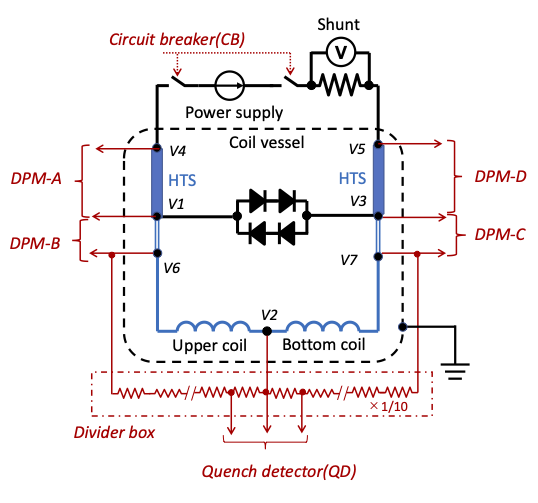
\includegraphics[width=0.6\textwidth]{fig/circuit.png}
  \caption{circuit}
  \label{fig:circuit}
\end{figure}

%% 図\ref{fig:result}に示すように...

\end{document}
